(I assume that I'm meant to build these in Keiko syntax)

Instruction sequence, commented with the stack, where \&s is the address of s:

\begin{lstlisting}
LOCAL -8  ! &s
LOADW     ! s
LOCAL -4  ! s; &q
LOADW     ! s; q
LOADW     ! s; q->data
PLUS      ! s + q->data
LOCAL -8  ! s + q->data; &s
STOREW    !
LOCAL -4  ! &q
LOADW     ! q
CONST 4   ! q; 4
OFFSET    ! q+4
LOADW     ! q->next
LOCAL -4  ! q->next, &q
STOREW
\end{lstlisting}

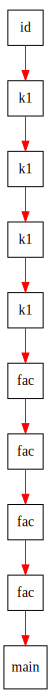
\includegraphics[width=\textwidth]{ex3.png}
